\chapter{Cryptographic Design}
%%%%%%%%%%%%%%%%%%%%%%%%%%%%%%%%%%%%%%%%%
\section{Introduction}
This chapter presents the cryptographic design of \projname{}, covering the core key concepts, key derivation flow, encryption algorithms, security properties, entropy sources, and the supplementary mouse randomness feature.

%%%%%%%%%%%%%%%%%%%%%%%%%%%%%%%%%%%%%%%%%
\section{Core Key Concepts}
%%%%%%%%%%%%%%%%%%%%%%%%%%%%%%%%%%%%%%%%%
The design uses two key concepts. The first is the \mvk{} \index{Master Vault Key}, a random 256-bit symmetric key that encrypts all vault data. The second is the \kek{} \index{Key Encryption Key}, a password-derived key created from the user's password using Argon2id. The \kek{} is used only to encrypt or decrypt the \mvk{} \cite{nist_keywrap, halevi_keywrap} and is never stored in plaintext.

%%%%%%%%%%%%%%%%%%%%%%%%%%%%%%%%%%%%%%%%%
\section{Key Derivation and Unlock Flow}
%%%%%%%%%%%%%%%%%%%%%%%%%%%%%%%%%%%%%%%%%
The unlock process is intentionally indirect. The password is never compared with a stored password hash for vault access. Instead, the system derives a \kek{} from the password and uses that key to decrypt the \mvk{}. If the decryption succeeds and the authentication tag verifies correctly, the password is accepted. If it fails, the password is rejected. The key derivation and unlock flow is shown in Figure \ref{fig:keyflow}.

\begin{figure}[h]
	\centering
	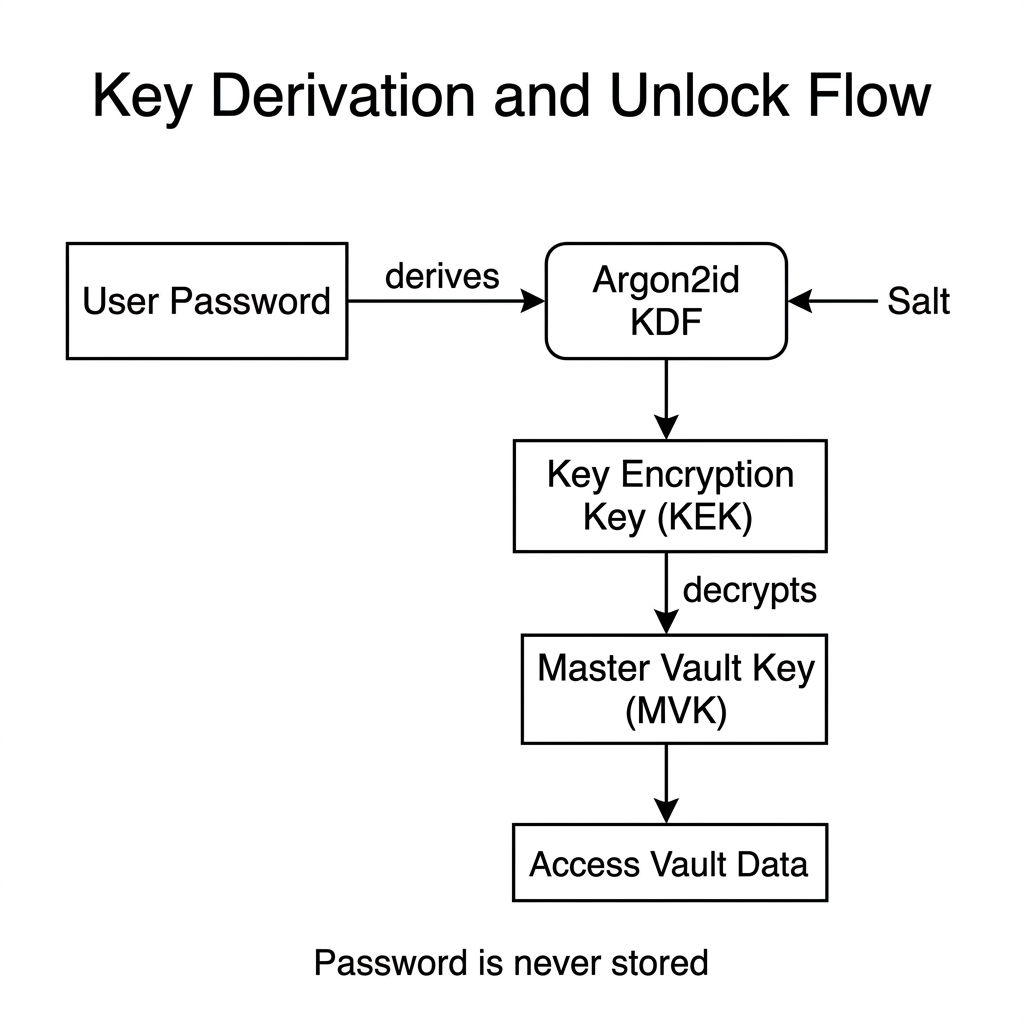
\includegraphics [width=0.85\textwidth] {figures/key_derivation_flow}
	\caption{Password-to-vault access flow. Authentication succeeds through correct cryptographic decryption rather than direct password comparison.}
	\label{fig:keyflow}	
\end{figure}

%%%%%%%%%%%%%%%%%%%%%%%%%%%%%%%%%%%%%%%%%
\section{AES-256-GCM}
%%%%%%%%%%%%%%%%%%%%%%%%%%%%%%%%%%%%%%%%%
AES-GCM \index{AES-256-GCM} \cite{nistaes, aes_fips197} is used because it provides confidentiality and integrity in a single mode of operation. AES-256 offers a strong key size, while GCM provides authenticated encryption with associated data \cite{rogaway_ae}. In the vault context, this means tampering with ciphertext is detected, and a modified encrypted blob will fail validation during decryption.

%%%%%%%%%%%%%%%%%%%%%%%%%%%%%%%%%%%%%%%%%
\section{Argon2id}
%%%%%%%%%%%%%%%%%%%%%%%%%%%%%%%%%%%%%%%%%
Argon2id \index{Argon2id} \cite{argon2} is a password-based key derivation function designed to be resistant to GPU and ASIC acceleration while also defending against tradeoffs between memory and computation. The project uses a memory cost of 64 MB, which raises the cost of brute-force attempts. The exact choice reflects a balance between security and usability on typical student hardware.

%%%%%%%%%%%%%%%%%%%%%%%%%%%%%%%%%%%%%%%%%
\section{Security Properties}
%%%%%%%%%%%%%%%%%%%%%%%%%%%%%%%%%%%%%%%%%
The cryptographic design provides several important properties:
\begin{itemize}
  \item the password is never stored in plaintext,
  \item there is no direct password comparison table,
  \item vault access is bound to successful authenticated decryption,
  \item encrypted container contents remain protected while stored,
  \item tampering with stored ciphertext is detected during decryption.
\end{itemize}

%%%%%%%%%%%%%%%%%%%%%%%%%%%%%%%%%%%%%%%%%
\section{Entropy Sources}
%%%%%%%%%%%%%%%%%%%%%%%%%%%%%%%%%%%%%%%%%
The system uses \texttt{SecureRandom} \index{SecureRandom} for cryptographic randomness. Optional mouse entropy can be mixed in as a supplementary source, but it is never the primary entropy source. Security is therefore not dependent on human motion or user behavior.

%%%%%%%%%%%%%%%%%%%%%%%%%%%%%%%%%%%%%%%%%
\section{Mouse Randomness Feature}
%%%%%%%%%%%%%%%%%%%%%%%%%%%%%%%%%%%%%%%%%

\subsection{Design Rationale}
Some implementations use user interaction data as an auxiliary entropy source. In \projname{}, mouse movements are optionally collected and converted to byte entropy. This design may improve entropy diversity, but it is carefully positioned as a supplementary feature only.

\subsection{Processing Model}
The application records mouse coordinates and timestamps, transforms them into bytes, and mixes them into the random generator through reseeding. Because cryptographic security must not depend on user behavior, this feature is not part of the trust base.

\subsection{Security Interpretation}
The feature must not be treated as primary entropy. If the mouse data were unavailable or predictable, the vault security would still rely on proper cryptographic primitives and a strong password. This distinction is important for honest security analysis.
